\chapter{Análisis y requisitos}\label{cap:especificación}

Antes de empezar con el desarrollo e implementación del sistema es necesario realizar una fase previa. En esta fase se 
van a extraer los requisitos que va a tener el sistema junto con las funcionalidades que tendrá. A 
continuación se va a explicar el proceso que se ha seguido.

\section{Recopilación de información}

Para recopilar información se ha recurrido a la realización de entrevistas, análisis de documentos y consultas a través
de correo electrónico con el personal adecuado.

\begin{itemize}
    \item \textbf{Entrevistas}
    \newline
    Se han realizado varias entrevistas con la finalidad de ajustar el sistema lo máximo posible a lo que se necesita
    o sería interesante que hubiese en el sector agrícola.

    \begin{itemize}
        \item \textbf{José Cobos Repiso - Agricultor de Cooperativa San Lorenzo de Zagra}
        \newline
        Con esta reunión se pudo ver cómo es el día a día de un agricultor que tiene varias fincas y cómo las gestiona.
        José mostró las distintas tablas que tiene creadas en Excel a través de las cuáles puede llevar un control exacto
        de qué actividad ha realizado en cada campaña y sobre qué finca en particular.
        Fueron varios los puntos planteados durante la reunión sobre qué podría tener la aplicación Olivaris. Entre
        ellos se destacaron:

        \begin{itemize}
            \item Funcionalidad de introducir un cuaderno de campo, siendo un punto muy interesante a tratar ya que el 
            próximo enero de 2027 va a ser obligatorio. Sobre esta funcionalidad se ha realizado un análisis más profundo
            que será comentado a continuación.
            \item Funcionalidad sobre control de costes y gastos, además de los pagos realizados a los empleados contratados.
            \item Funcionalidad sobre gestionar parcelas y las actividades realizadas en cada una de ellas, de manera que 
            se tenga una vista de todas las parcelas que son de su propiedad y se puedan gestionar las actividades de cada una
            de ellas. 
        \end{itemize}

        Gracias a este reunión se pudo obtener una aproximación de qué tipo de tablas se tendrían en la base de datos,
        cómo se podrían relacionar entre ellas y que funcionalidades tendría la aplicación.

        \item \textbf{Juan Luis Jiménez Laredo - Profesor titular de la ETSIIT y Director del presente TFG}
        \newline
        Las reuniones realizadas con Juan Luis han servido para llevar una revisión continua del desarrollo del proyecto,
        con la finalidad de saber qué requisitos funcionales tendrá el sistema y qué tareas hay que priorizar.
        Además, contando también con experiencia en el sector de la oliva, ha podido dar una visión del sistema más precisa,
        siendo esto de gran ayuda para definir cuáles son las funcionalidades más relevantes de la aplicación.

        Con la información extraída de la reunión realizada con José sobre el cuaderno de campo y con las conversaciones
        mantenidas con Juan Luis, se exploró la opción de introducir la funcionalidad del cuaderno de campo digital. 
        
        El \textbf{cuaderno de campo \cite{cuadernoCampo}} es una especie de cuaderno de bitácora que registra el uso 
        de productos químicos (fitosanitarios y fertilizantes) sobre una explotación con la finalidad de vigilar la 
        posible contaminación que pueda surgir derivada del abuso de estos productos. Este concepto está muy relacionado
        con el \textbf{Cuaderno Digital de Explotación Agrícola (CUE)}.

        Según la Conserjería de Agricultura, Pesca, Agua y Desarrollo Rural \cite{cueDigital}, el Cuaderno Digital de 
        Explotación Agrícola (o CUE digital), es la herramienta que se va a utilizar en España para anotar las 
        actividades que se realizan en una explotación agrícola, recogiendo las actividades fitosanitarias, de 
        fertilización o riegos aplicados. Para poder cumplimentar este CUE digital, es necesario que la explotación este
        previamente inscrita en REAFA (Registro Autonómico de Explotaciones Agrarias en Andalucía), ya que esta será la 
        fuente que proporcione la información de las parcelas y cultivos existentes.

        Este CUE digital, a diferencia del CUE de papel, obliga a que sea tratado desde medios electrónicos y que la
        información que lo cumplimente sea con los datos que la Administración tenga disponibles, procedentes del 
        Registro Autonómico de Explotaciones (REA).

        El aspecto que hace interesante la implementación de esta funcionalidad es que a partir del 1 de enero de 2027
        será obligatorio el uso del CUE digital para consignar la información de los tratamientos fitosanitarios. 
        
        A partir de este punto, se ha realizado una búsqueda de cómo acceder a la API que proporciona la Junta de 
        Andalucía para obtener los datos de una explotación y poder exportarlos al CUE digital. Para ello, primero es
        necesario dar de alta la ``empresa'' que va a desarrollar este proyecto en un portal junto con su certificado
        digital, estando aquí el primer problema: actualmente no hay constituida una empresa de desarrollo de software 
        particular, por lo que no hay certificado digital que se pueda utilizar para darse de alta y poder acceder a la
        API.

        Las soluciones buscadas han conllevado el envío de correos electrónicos a entidades que puedan suplir este problema
        y hacer de ``empresa de desarrollo''. Los correos enviados se van a comentar a continuación.
    \end{itemize}

    \item \textbf{Correos electrónicos}
    \newline
    Se han enviado correos electrónicos a las siguientes entidades, con la finalidad de buscar ayuda para dar de alta
    una empresa en el sistema y poder obtener el certificado digital que permita acceder a la API.

    \begin{itemize}
        \item \textbf{Nomia Energy}: empresa de Granada con la que se ha contactado para darla de alta en el registro
        como empresa desarrolladora del Cuaderno Digital de Explotación comercial. Con su certificado digital se podría
        acceder a la API pero finalmente no se llegó a un acuerdo y esta opción se descartó.

        \item \textbf{Trabajador de la Junta de Andalucía}: se mantuvieron conversaciones con Juan Carlos Martín Fuentes,
        trabajador de la Junta de Andalucía, para recoger qué requisitos son necesarios para registrarse como empresa de 
        desarrollo y sobre cómo tiene que ser el certificado digital, ya que se contempló la opción de trabajar con un 
        certificado ``autofirmado'' en el entorno de prepoducción (por no tener una empresa que proporcione el certificado), 
        pero finalmente esta opción se descartó porque no admiten certificados autofirmados, debido a la poca fiabilidad que
        tienen.        

        \item \textbf{Jefe de Seguridad de los Servicios Informáticos de la UGR}: se contactó con el Jefe de Seguridad
        para comentarle qué situación había, qué se quería realizar y cómo es el tipo de certificado digital que se 
        necesita para poder acceder a esta API. Se comentó las partes que deben incluir el certificado: parte pública 
        en formato .PEM, \hyperlink{certificadoTls}{\textit{TLS Web Client Authentiacion}} (clientAuth) y el 
        subdominio de la entidad o el CIF/NIF (el de la UGR en este caso), con la finalidad de saber si la UGR puede 
        gestionar un certificado con estas características y de esta forma poder acceder al sistema.
    \end{itemize}

    La funcionalidad del CUE digital es muy interesante pero ha tenido un problema: el proceso para extraer la información 
    es largo y lento (muchos correos electrónicos y tiempos de espera entre ellos), así como problemas derivados del uso de 
    un certificado digital que no se tiene, por lo que esta funcionalidad ha pasado a un segundo plano. El proyecto se ha 
    centrado en desarrollar el sistema con una base de datos y lógica de negocio propia que ``supla'' la falta de acceso a los
    endpoints de la API que se encargarían de realizar estas acciones.
\end{itemize}

\section{CUE comercial}

Durante esta fase de análisis, viendo la necesidad que va a haber a partir de enero del próximo año 2027 en facilitar un CUE comercial 
(aplicación software) a los titulares de una explotación, se ha orientado el desarrollo del sistema hacia este ámbito. Esta 
decisión ha causado que el sistema evolucione de un ERP clásico que se iba a desarrollar en un principio, a acotar el sistema 
a un diario de actividades que permita registrar su información en un CUE digital utilizando los datos suministrados por el usuario
y por la REA (en caso de poder acceder a la API).

A partir de este punto, el sistema a desarrollar debe poder acceder a la API o interfaz que suministran el \textbf{SIEX} (Sistema de Información
de Explotaciones Agrarias) para consumir sus endpoints, permitiendo obtener datos de la REA y exportar datos al CUE digital. Sin embargo, este 
proceso empezó siendo lento y tedioso, ya que requería un certificado que como se ha comentado antes, ha sido difícil de conseguir, por lo que se 
tomó la decisión de elaborar un sistema con una base de datos propia, que tenga las entidades necesarias para almacenar la información que podrían 
rellenar los datos del CUE digital. De esta manera, el sistema también estaría adaptado a una posible integración futura de la API, ya que sería añadir
el cliente de esta y que los datos sean enviados directamente a los servidores del REA y CUE que maneja el ministerio en vez de almacenarlos en las tablas.

Para obtener información sobre el CUE, se han accedido a los siguientes anexos principalmente:

\begin{itemize}
    \item \textbf{Anexo IX - Modelo de autorización de acceso a la información del REA y CUE:} este anexo se ha utilizado para saber qué permisos son
    los que cede un usuario que pertenece a una entidad habilitada sobre dicha entidad. Además de este, también se ha utilizado el anexo \textbf{Anexo VIII - 
    Modelo de Autorización de Representación} para investigar sobre los permisos.

    \item \textbf{Anexo VI - Interfaz Único Común:} este anexo se ha utilizado para comprender cómo funciona la interfaz de acceso o API. Como al final no 
    se pudo acceder a ella, la consulta a este anexo fue al inico del proyecto y sin entrar en detalle.

    \item \textbf{Anexo X - Registro de Autorizaciones para el uso de Aplicaciones Comerciales:} este anexo ha servido para comprender qué tipo de usuarios 
    van a interactuar con la aplicación y entre ellos, pudiendo distinguir entre tres: empresa desarrollador del software, entidad habilitada y titular de la
    explotación.

    \item \textbf{Anexo III - Registros de los tratamientos fitosanitarios y de fertilización:} este anexo se ha utilizado para investigar sobre qué datos de una
    explotación así como de una actividad fitosanitaria son utilizados para el cuaderno de explotación.
\end{itemize}

Otras fuentes que se visitaron para obtener más información fue el \textbf{Cuaderno de Explotación de la Junta de Andalucía}. En esta página se ha consultado 
información sobre el CUE Comercial (aplicación desarrollada), como por ejemplo: la fecha en la que será obligatorio el uso del CUE Digital para los agricultores 
en las actividades de tipo fitosanitario, o el proceso que tiene que seguir una empresa para darse de alta como CUE Comercial y poder acceder a la interfaz IUWS.

\section{Personas}

Una parte muy importante durante el análisis de un sistema son los usuarios finales que lo utilizan. Por ello, se han creado
personas ficticias que puedan representar al usuario que utiliza la aplicación, consiguiendo saber de esta manera cuáles son 
sus inquietudes y qué necesitan para poder realizar sus tareas correctamente.

En las imágenes \ref{fig:persona_1} y \ref{fig:persona_2} se muestran los tipos de usuarios que se han elaborado según las 
necesidades de la aplicación.

\begin{figure}[H]
    \centering
    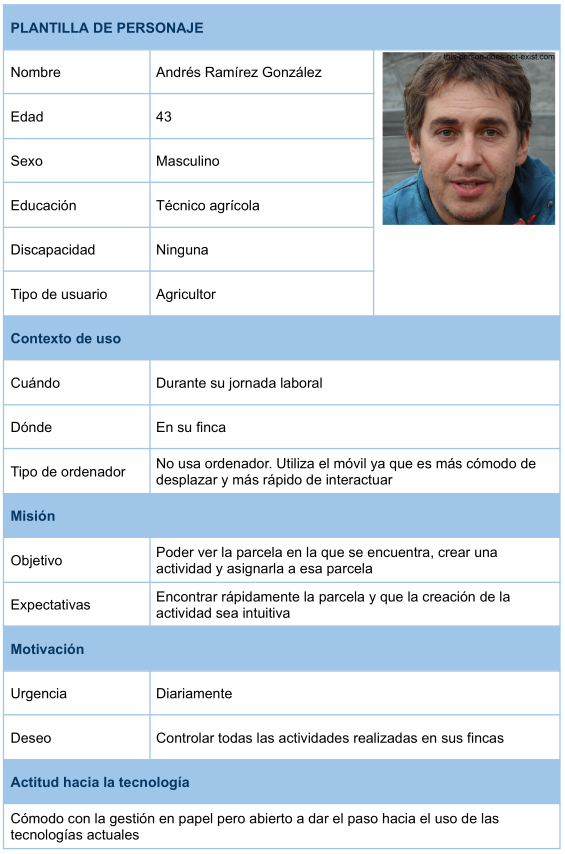
\includegraphics[width=0.8\textwidth]{figures/03_persona1.png}
    \caption{Persona 1: Agricultor}
    \label{fig:persona_1}
\end{figure}

\begin{figure}[H]
    \centering
    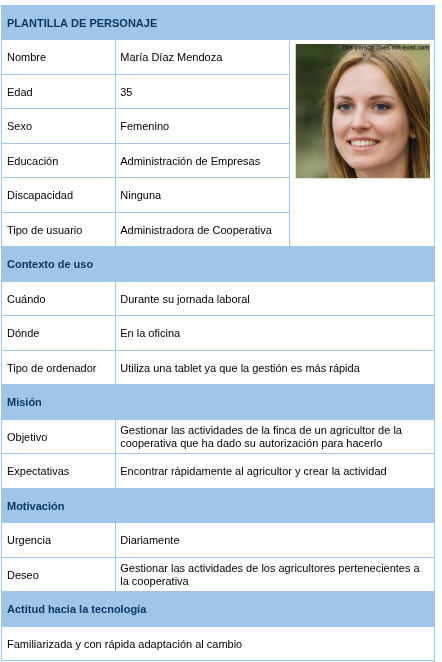
\includegraphics[width=0.8\textwidth]{figures/03_persona2.png}
    \caption{Persona 2: Administradora de la Cooperativa}
    \label{fig:persona_2}
\end{figure}

\section{Escenarios}

Una vez que han sido planteadas las personas, se pasa a describir los escenarios. Los escenarios son una descripción de
como el usuario utiliza el sistema para realizar una determinada tarea y lograr su objetivo. A través de esta técnica se
consigue ver de una forma más clara y cercana cómo debe de funcionar el sistema, pudiendo ayudar a encontrar y definir
requisitos funcionales.

Los escenarios planteados para las personas creadas en el apartado anterior son los siguientes:

\begin{itemize}
    \item \textbf{Primer escenario: Andrés Ramírez González (Agricultor)}
    \newline
    Andrés se encuentra realizando su jornada laboral en una de sus fincas y utiliza su móvil como herramienta principal 
    ya que necesita rapidez y se está moviendo constantemente.

    Andrés abre la aplicación y esta muestra un mapa con la geolocalización actual y las parcelas de su finca bien
    delimitadas. Procede a pulsar en una parcela y el sistema muestra información básica sobre la finca y un botón que le
    permite crear una actividad nueva asociada a esa parcela. Andrés selecciona esta opción y el sistema le envía a una 
    página que muestra un sencillo e intuitivo formulario que debe rellenar indicando el tipo de actividad que va a crear.

    Una vez guardada la información en el sistema, se muestra un mensaje de confirmación y se asocia automáticamente a la 
    parcela, pudiendo resivar Andrés el historial de actividades de esa finca en cualquier momento y controlando todo el 
    trabajo realizado en cualquier momento sin necesidad de papel.

    \begin{itemize}
        \item \textbf{Valor añadido}: identificación rápida de la parcela, creación de actividades de forma ágil y control
        centralizado de todas las tareas.
    \end{itemize}

    \item \textbf{Segundo escenario: María Díaz Mendoza (Administradora de Cooperativa)}
    \newline
    María se encuentra la oficina durante su jornada laboral, utilizando una tablet para gestionar de forma rápida y 
    eficiente tanto las fincas como actividades de los agricultores.

    María accede a la aplicación con su perfil de administradora de cooperativa y el sistema le muestra una lista con 
    todos los agricultores asociados que han autorizado la gestión de sus fincas, por lo que procede a seleccionar uno de ellos
    y el sistema le muestra una vista con todas las actividades asociadas a ese agricultor.

    María quiere añadir una nueva actividad por lo que pulsa sobre el botón que agrega una actividad. A continuación,
    se le presenta un formulario que debe de rellenar según la actividad a realizar.

    Una vez rellenado y guardado, el sistema la almacena automáticamente y la asocia a la parcela, quedando registrada para una
    consulta posterior tanto por María como por un agricultor. Este proceso se podrá repetir tantas veces como sea necesario con 
    distintos agricultores, asegurando una gestión centralizada y organizada.

    \begin{itemize}
        \item \textbf{Valor añadido}: gestión remota de varias fincas autorizadas, acceso rápido a las actividades y
        mejora de la coordinación y trazabilidad entre cooperativa y agricultores. 
    \end{itemize}
\end{itemize}

\section{Historias de Usuario}

Una \textbf{Historia de Usuario} \cite{historiaUsuario} es una descripción general e informal de una función de software escrita 
desde la persepectiva del usuario final o cliente. Su propósito es describir cómo un elemento de trabajo aporta un valor 
particular al cliente.

Son redactadas con un lenguaje sencillo y no técnico y consiguen con pocas palabras describir el resultado deseado. A partir de 
ellas se pueden establacer los requisitos funcionales del sistema y son añadidas a las iteraciones o \textit{sprints} dentro de 
la metodología ágil \hyperlink{scrum}{Scrum}.

Las historias de usuario son importantes ya que ayudan a los equipos de trabajo a centrarse en solucionar problemas para
usuarios reales, a que piensen de forma crítica y creativa sobre cómo lograr una meta de forma eficaz y ayudan a 
motivar al equipo ya que su resolución implica pequeños retos y victorias.

Para la realización de las Historias de Usuario del presente proyecto, la estructura utilizada ha sido la siguiente:

\textit{\textbf{Como} [tipo de usuario que realiza la acción], \textbf{quiero} [la acción que se quiere realizar] \textbf{para} 
[resultado obtenido].}

Además de la historia de usuario, se ha añadido el identificador de esa historia de usuario y un título identificativo.

Según los análisis realizados y la información obtenida, se han establecido las siguientes historias de usuario:

\begin{table}[H]
    \centering
    \begin{tabular}{|p{2cm}|p{4cm}|p{2cm}|p{4cm}|}
        \hline
        \textbf{ID} & HU-1 & \textbf{Nombre} & Inicio de sesión \\
        \hline
        \multicolumn{2}{|p{6cm}|}{\textbf{Descripción}} & \multicolumn{2}{p{6cm}|}{Como usuario, quiero iniciar sesión en la aplicación para acceder de forma segura a mis datos.} \\
        \hline
    \end{tabular}
    \caption{Historia de usuario HU-1}
    \label{tab:hu_1}
\end{table}

\begin{table}[H]
    \centering
    \begin{tabular}{|p{2cm}|p{4cm}|p{2cm}|p{4cm}|}
        \hline
        \textbf{ID} & HU-2 & \textbf{Nombre} & Sesión segura \\
        \hline
        \multicolumn{2}{|p{6cm}|}{\textbf{Descripción}} & \multicolumn{2}{p{6cm}|}{Como usuario, quiero que mi sesión sea segura para evitar accesos no autorizados.} \\
        \hline
    \end{tabular}
    \caption{Historia de usuario HU-2}
    \label{tab:hu_2}
\end{table}

\begin{table}[H]
    \centering
    \begin{tabular}{|p{2cm}|p{4cm}|p{2cm}|p{4cm}|}
        \hline
        \textbf{ID} & HU-3 & \textbf{Nombre} & Asignación de roles \\
        \hline
        \multicolumn{2}{|p{6cm}|}{\textbf{Descripción}} & \multicolumn{2}{p{6cm}|}{Como administrador, quiero asignar roles a los usuarios para controlar qué puede hacer cada uno.} \\
        \hline
    \end{tabular}
    \caption{Historia de usuario HU-3}
    \label{tab:hu_3}
\end{table}

\begin{table}[H]
    \centering
    \begin{tabular}{|p{2cm}|p{4cm}|p{2cm}|p{4cm}|}
        \hline
        \textbf{ID} & HU-4 & \textbf{Nombre} & Control de funcionalidad según rol \\
        \hline
        \multicolumn{2}{|p{6cm}|}{\textbf{Descripción}} & \multicolumn{2}{p{6cm}|}{Como administrador, quiero que el sistema controle el acceso a cada funcionalidad según el rol para evitar manipulación indeseada de datos.} \\
        \hline
    \end{tabular}
    \caption{Historia de usuario HU-4}
    \label{tab:hu_4}
\end{table}

\begin{table}[H]
    \centering
    \begin{tabular}{|p{2cm}|p{4cm}|p{2cm}|p{4cm}|}
        \hline
        \textbf{ID} & HU-5 & \textbf{Nombre} & Registro de entidades habilitadas \\
        \hline
        \multicolumn{2}{|p{6cm}|}{\textbf{Descripción}} & \multicolumn{2}{p{6cm}|}{Como usuario quiero registrar una entidad en el sistema para que se puedan gestionar los datos de los usuarios que pertenezcan a ella.} \\
        \hline
    \end{tabular}
    \caption{Historia de usuario HU-5}
    \label{tab:hu_5}
\end{table}

\begin{table}[H]
    \centering
    \begin{tabular}{|p{2cm}|p{4cm}|p{2cm}|p{4cm}|}
        \hline
        \textbf{ID} & HU-6 & \textbf{Nombre} & Control de actividades \\
        \hline
        \multicolumn{2}{|p{6cm}|}{\textbf{Descripción}} & \multicolumn{2}{p{6cm}|}{Como entidad habilitada, quiero gestionar las fincas y sus actividades para que el agricultor no tenga que realizar estas tareas.} \\
        \hline
    \end{tabular}
    \caption{Historia de usuario HU-6}
    \label{tab:hu_6}
\end{table}

\begin{table}[H]
    \centering
    \begin{tabular}{|p{2cm}|p{4cm}|p{2cm}|p{4cm}|}
        \hline
        \textbf{ID} & HU-7 & \textbf{Nombre} & Gestión de parcelas \\
        \hline
        \multicolumn{2}{|p{6cm}|}{\textbf{Descripción}} & \multicolumn{2}{p{6cm}|}{Como agricultor, quiero registrar una parcela con sus datos para poder gestionarla correctamente.} \\
        \hline
    \end{tabular}
    \caption{Historia de usuario HU-7}
    \label{tab:hu_7}
\end{table}

\begin{table}[H]
    \centering
    \begin{tabular}{|p{2cm}|p{4cm}|p{2cm}|p{4cm}|}
        \hline
        \textbf{ID} & HU-8 & \textbf{Nombre} & Registro de actividades \\
        \hline
        \multicolumn{2}{|p{6cm}|}{\textbf{Descripción}} & \multicolumn{2}{p{6cm}|}{Como agricultor, quiero registrar una actividad diaria para llevar un control centralizado.} \\
        \hline
    \end{tabular}
    \caption{Historia de usuario HU-8}
    \label{tab:hu_8}
\end{table}

\begin{table}[H]
    \centering
    \begin{tabular}{|p{2cm}|p{4cm}|p{2cm}|p{4cm}|}
        \hline
        \textbf{ID} & HU-9 & \textbf{Nombre} & Registro de actividad fitosanitaria \\
        \hline
        \multicolumn{2}{|p{6cm}|}{\textbf{Descripción}} & \multicolumn{2}{p{6cm}|}{Como agricultor, quiero registrar un tratamiento fitosanitario para cumplir la normativa.} \\
        \hline
    \end{tabular}
    \caption{Historia de usuario HU-9}
    \label{tab:hu_9}
\end{table}

\begin{table}[H]
    \centering
    \begin{tabular}{|p{2cm}|p{4cm}|p{2cm}|p{4cm}|}
        \hline
        \textbf{ID} & HU-10 & \textbf{Nombre} & Registro de actividad futura o planificada \\
        \hline
        \multicolumn{2}{|p{6cm}|}{\textbf{Descripción}} & \multicolumn{2}{p{6cm}|}{Como agricultor, quiero planificar actividades futuras para organizar el trabajo de la campaña.} \\
        \hline
    \end{tabular}
    \caption{Historia de usuario HU-10}
    \label{tab:hu_10}
\end{table}

\begin{table}[H]
    \centering
    \begin{tabular}{|p{2cm}|p{4cm}|p{2cm}|p{4cm}|}
        \hline
        \textbf{ID} & HU-11 & \textbf{Nombre} & Modificación de actividad \\
        \hline
        \multicolumn{2}{|p{6cm}|}{\textbf{Descripción}} & \multicolumn{2}{p{6cm}|}{Como agricultor, quiero modificar una actividad almacenada para corregir datos o marcarla como realizada.} \\
        \hline
    \end{tabular}
    \caption{Historia de usuario HU-11}
    \label{tab:hu_11}
\end{table}

\begin{table}[H]
    \centering
    \begin{tabular}{|p{2cm}|p{4cm}|p{2cm}|p{4cm}|}
        \hline
        \textbf{ID} & HU-12 & \textbf{Nombre} & Eliminación de actividad \\
        \hline
        \multicolumn{2}{|p{6cm}|}{\textbf{Descripción}} & \multicolumn{2}{p{6cm}|}{Como agricultor, quiero eliminar una actividad para no tenerla guardada en el sistema.} \\
        \hline
    \end{tabular}
    \caption{Historia de usuario HU-12}
    \label{tab:hu_12}
\end{table}

\begin{table}[H]
    \centering
    \begin{tabular}{|p{2cm}|p{4cm}|p{2cm}|p{4cm}|}
        \hline
        \textbf{ID} & HU-13 & \textbf{Nombre} & Control de usuarios \\
        \hline
        \multicolumn{2}{|p{6cm}|}{\textbf{Descripción}} & \multicolumn{2}{p{6cm}|}{Como administrador, quiero obtener los usuarios registrados en el sistema para llevar un control de quien está registrado.} \\
        \hline
    \end{tabular}
    \caption{Historia de usuario HU-13}
    \label{tab:hu_13}
\end{table}

\begin{table}[H]
    \centering
    \begin{tabular}{|p{2cm}|p{4cm}|p{2cm}|p{4cm}|}
        \hline
        \textbf{ID} & HU-14 & \textbf{Nombre} & Consulta de parcela \\
        \hline
        \multicolumn{2}{|p{6cm}|}{\textbf{Descripción}} & \multicolumn{2}{p{6cm}|}{Como agricultor, quiero consultar mis parcelas, para obtener información sobre ellas.} \\
        \hline
    \end{tabular}
    \caption{Historia de usuario HU-14}
    \label{tab:hu_14}
\end{table}

\begin{table}[H]
    \centering
    \begin{tabular}{|p{2cm}|p{4cm}|p{2cm}|p{4cm}|}
        \hline
        \textbf{ID} & HU-15 & \textbf{Nombre} & Consulta de actividades \\
        \hline
        \multicolumn{2}{|p{6cm}|}{\textbf{Descripción}} & \multicolumn{2}{p{6cm}|}{Como agricultor, quiero consultar el historial de actividades de un usuario para saber todo lo que ha realizado.} \\
        \hline
    \end{tabular}
    \caption{Historia de usuario HU-15}
    \label{tab:hu_15}
\end{table}

\begin{table}[H]
    \centering
    \begin{tabular}{|p{2cm}|p{4cm}|p{2cm}|p{4cm}|}
        \hline
        \textbf{ID} & HU-16 & \textbf{Nombre} & Visualización de parcelas en un mapa \\
        \hline
        \multicolumn{2}{|p{6cm}|}{\textbf{Descripción}} & \multicolumn{2}{p{6cm}|}{Como agricultor, quiero visualizar mis parcelas en un mapa para conocer rápidamente el estado de las tareas.} \\
        \hline
    \end{tabular}
    \caption{Historia de usuario HU-16}
    \label{tab:hu_16}
\end{table}

\begin{table}[H]
    \centering
    \begin{tabular}{|p{2cm}|p{4cm}|p{2cm}|p{4cm}|}
        \hline
        \textbf{ID} & HU-17 & \textbf{Nombre} & Cierre de sesión \\
        \hline
        \multicolumn{2}{|p{6cm}|}{\textbf{Descripción}} & \multicolumn{2}{p{6cm}|}{Como usuario, quiero cerrar sesión para proteger mis datos cuando dejo de usar la aplicación.} \\
        \hline
    \end{tabular}
    \caption{Historia de usuario HU-17}
    \label{tab:hu_17}
\end{table}

\begin{table}[H]
    \centering
    \begin{tabular}{|p{2cm}|p{4cm}|p{2cm}|p{4cm}|}
        \hline
        \textbf{ID} & HU-18 & \textbf{Nombre} & Registro de actividades \\
        \hline
        \multicolumn{2}{|p{6cm}|}{\textbf{Descripción}} & \multicolumn{2}{p{6cm}|}{Como agricultor, quiero registrar una actividad directamente desde el mapa para agilizar el trabajo en campo.} \\
        \hline
    \end{tabular}
    \caption{Historia de usuario HU-18}
    \label{tab:hu_18}
\end{table}

\section{Criterios de aceptación}

Las historias de usuario definidas tienen unos criterios de aceptación asociados que establecen cuando una historia de usuario ha sido
completada. Los criterios de aceptación para cada historia de usuario son los siguientes:

\begin{itemize}
    \item \textbf{HU-01}
    \begin{itemize}
        \item Dado que introduzco usuario/email y contraseña correctos, cuando inicio sesión, entonces accedo a la aplicación.
        \item Dado que no he confirmado mi registro, cuando inicio sesión, el sistema no me lo permite.
        \item Dado que introduzco credenciales incorrectas, cuando intento iniciar sesión, entonces el sistema muestra un mensaje de error.
        \item Dado que no estoy autenticado, cuando intento acceder a una funcionalidad protegida, el sistema no me lo permite.
    \end{itemize}
\end{itemize}

\begin{itemize}
    \item \textbf{HU-02}
    \begin{itemize}
        \item Dado que inicio sesión, cuando pasa el tiempo de inactividad configurado, entonces la sesión expira.
        \item Dado que la sesión expira, cuando intento continuar, entonces debo volver a autenticarme.
    \end{itemize}
\end{itemize}

\begin{itemize}
    \item \textbf{HU-03}
    \begin{itemize}
        \item Dado que un usuario tiene un rol asignado, cuando accede al sistema, entonces solo puede realizar lo permitido.
    \end{itemize}
\end{itemize}

\begin{itemize}
    \item \textbf{HU-04}
    \begin{itemize}
        \item Dado que intento realizar una acción no permitida en base a mi rol, entonces el sistema lo bloquea.
    \end{itemize}
\end{itemize}

\begin{itemize}
    \item \textbf{HU-05}
    \begin{itemize}
        \item Un usuario con rol de administrador puede crear una entidad habilitada en el sistema.
        \item El sistema impedirá que un usuario con otro rol quiera registrar una entidad.
        \item Los campos de nombre, NIF y correo electrónico son obligatorios; sin ellos no se podrá crear la entidad.
    \end{itemize}
\end{itemize}

\begin{itemize}
    \item \textbf{HU-06}
    \begin{itemize}
        \item El sistema no permite que un usuario con rol administrador dentro de una entidad pueda manipular datos de usuarios que no le han dado permiso.
        \item El sistema no permite que un usuario pueda gestionar datos o usuarios de otras entidades a las que no pertenece.
        \item Un usuario que pertenece a una entidad con rol administrador podrá gestionar las actividades de otro usuario que haya otorgado permisos dentro 
        de la misma entidad.
    \end{itemize}
\end{itemize}

\begin{itemize}
    \item \textbf{HU-07}
    \begin{itemize}
        \item Dado que introduzco los datos válidos de una parcela, cuando la guardo, entonces la parcela queda registrada en el sistema.
        \item Dado que la parcela tiene recintos, cuando se guarda la parcela, entonces los recintos quedan almacenados y vinculados a la parcela.
        \item Dado que faltan datos obligatorios de la parcela, cuando intento guardarla, entonces el sistema muestra un error indicando los campos inválidos.
        \item Dado que existen recintos con datos inválidos o incompletos, cuando intento guardar la parcela, entonces el sistema muestra un error.
    \end{itemize}
\end{itemize}

\begin{itemize}
    \item \textbf{HU-08}
    \begin{itemize}
        \item Dado que introduzco datos válidos de una actividad, cuando la guardo, entonces la actividad queda registrada en el sistema.
        \item Dado que la actividad tiene estado ``Completada'', cuando introduzco una fecha futura, entonces el sistema muestra un error.
        \item Dado que falta alguno de los campos obligatorios (fecha, campaña, parcela/recinto o tipo de actividad), cuando intento guardar, entonces el 
        sistema muestra un error indicando los campos inválidos.
        \item Dado que la parcela o recinto no existe, cuando intento registrar la actividad, entonces el sistema muestra un error.
        \item Dado que el usuario es admin dentro de una entidad, cuando registra una actividad para otro usuario de su entidad con permisos, entonces la 
        actividad se guarda correctamente.
        \item Dado que el usuario es ``agricultor'' o ``administrador'' y no pertenecen a ninguna entidad con rol ``agricultor'', cuando registra una actividad, 
        entonces solo puede hacerlo para sí mismo.
    \end{itemize}
\end{itemize}

\begin{itemize}
    \item \textbf{HU-09}
    \begin{itemize}
        \item Dado que selecciono el tipo de actividad ``fitosanitaria'', cuando accedo al formulario de registro, entonces el sistema solicita los campos 
        necesarios como dosis, NIF del aplicador, fecha y tipo de cultivo.
        \item Dado que introduzco todos los datos válidos de un tratamiento fitosanitario, cuando guardo la actividad, entonces el tratamiento queda registrado 
        en el sistema y asociado a la actividad.
        \item Dado que falta alguno de los campos obligatorios cuando intento guardar, entonces el sistema muestra un error indicando los campos inválidos.
        \item Dado que registro un tratamiento fitosanitario válido, cuando se guarda la actividad, entonces se almacena en la tabla de actividades y en la 
        tabla específica de tratamientos.
    \end{itemize}
\end{itemize}

\begin{itemize}
    \item \textbf{HU-10}
    \begin{itemize}
        \item Dado que introduzco los datos válidos de una actividad con fecha futura, cuando la guardo, entonces la actividad queda registrada en el sistema 
        como ``Planificada''.
        \item Dado que intento registrar una actividad planificada, cuando introduzco una fecha pasada, entonces el sistema muestra un error.
        \item Dado que no se ha insertado una campaña, cuando intento guardar la actividad, entonces el sistema muestra un error. 
    \end{itemize}
\end{itemize}

\begin{itemize}
    \item \textbf{HU-11}
    \begin{itemize}
        \item Dado que existe una actividad registrada, cuando modifico sus datos con valores válidos y guardo, entonces la actividad se actualiza correctamente 
        en el sistema.
        \item Dado que falta algún campo obligatorio tras la modificación, cuando intento guardar los cambios, entonces el sistema muestra un error.
        \item Dado que se modifica el estado de una actividad ``completada'' a ``planificada'', el sistema muestra un error. 
    \end{itemize}
\end{itemize}

\begin{itemize}
    \item \textbf{HU-12}
    \begin{itemize}
        \item Dado que elimino una actividad, si esta existe, entonces desaparece.
        \item Dado que la actividad contenía datos en tablas específicas, entonces los datos asociados se eliminan o recalculan.
    \end{itemize}
\end{itemize}

\begin{itemize}
    \item \textbf{HU-13}
    \begin{itemize}
        \item Dado que el usuario tiene rol ``administrador'', cuando accede al listado de usuarios, entonces el sistema muestra 
        todos los usuarios registrados.
        \item Dado que el usuario no tiene rol ``administrador'', cuando intenta acceder al listado de usuarios, entonces el 
        sistema deniega el acceso.
        \item Dado que accedo al listado de usuarios, cuando se muestran los resultados, entonces veo los datos básicos de 
        cada usuario (nombre, email, rol y estado).
    \end{itemize}
\end{itemize}

\begin{itemize}
    \item \textbf{HU-14}
    \begin{itemize}
        \item Dado que el usuario existe en el sistema, puede acceder a la información de sus parcelas.
        \item Dado que el usuario tiene la parcela asignada, entonces se muestra la información de ella.
    \end{itemize}
\end{itemize}

\begin{itemize}
    \item \textbf{HU-15}
    \begin{itemize}
        \item Dado que el historial de actividades es de un usuario distinto del que las quiere obtener, 
        en caso de no tener rol de administrador dentro de la misma entidad el sistema lo impedirá.
    \end{itemize}
\end{itemize}

\begin{itemize}
    \item \textbf{HU-16}
    \begin{itemize}
        \item Dado que el usuario existe, el sistema obtiene las parcelas asignadas a el y las dibuja 
        sobre un mapa.
    \end{itemize}
\end{itemize}

\begin{itemize}
    \item \textbf{HU-17}
    \begin{itemize}
        \item Dado que he iniciado sesión en el sistema, cuando cierro sesión, los tokens que me permiten
        el acceso son eliminados y no puedo acceder al sistema.
        \item Dado que la sesión ha sido cerrada, hay que iniciar sesión de nuevo para poder acceder al sistema.
    \end{itemize}
\end{itemize}

\begin{itemize}
    \item \textbf{HU-18}
    \begin{itemize}
        \item Dado que la parcela y el recinto aparece dibujado en el mapa, cuando el usuario clicka en ella,
        aparece un enlace al formulario de registro.
        \item Dado que se registra correctamente la actividad, queda almacenada en las tablas del sistema.
    \end{itemize}
\end{itemize}

\section{Requisitos funcionales}

Los requisitos funcionales sirven para indicar qué funciones tiene el sistema y qué debe hacer. A partir 
de las historias de usuario se han extraído los siguientes requisitos funcionales agrupados por áreas. 
La estructura es del tipo \textit{RF-[ID de HU].XX}.

\subsection{Autenticación y autorización}

\begin{itemize}
    \item \textbf{RF-01.1)} El sistema debe permitir autenticación mediante usuario/email y contraseña.
    \item \textbf{RF-01.2)} El sistema debe validar las credenciales contra la base de datos.
    \item \textbf{RF-01.3)} El sistema debe iniciar una sesión de usuario tras autenticación correcta.
    \item \textbf{RF-01.4)} El sistema debe impedir el acceso a usuarios no autenticados.
    \item \textbf{RF-02.1)} El sistema debe gestionar expiración de sesiones o tokens.
    \item \textbf{RF-02.2)} El sistema debe invalidar sesiones antiguas automáticamente.
    \item \textbf{RF-02.3)} El sistema debe proteger endpoints con autenticación obligatoria.
    \item \textbf{RF-03.1)} El sistema debe soportar al menos los roles: administrador, entidad habilitada (cooperativa), agricultor.
    \item \textbf{RF-03.2)} El sistema debe evaluar permisos en función del rol del usuario.
    \item \textbf{RF-03.3)} El sistema debe ocultar o deshabilitar funcionalidades no autorizadas.
    \item \textbf{RF-04.1)} El sistema debe validar permisos antes de ejecutar cualquier acción.
    \item \textbf{RF-04.2)} El sistema debe impedir operaciones no autorizadas a nivel de backend.
    \item \textbf{RF-17.1)} El sistema debe eliminar los tokens guardados del usuario para evitar futuras peticiones.
    \item \textbf{RF-17.2)} El sistema debe mostrar la página de inicio de sesión en caso de haber cerrido la sesión.
\end{itemize}

\subsection{Entidades habilitadas}

\begin{itemize}
    \item \textbf{RF-05.1)} El sistema debe permitir registrar una entidad habilitada en el sistema si los campos son correctos.
    \item \textbf{RF-05.2)} El sistema debe impedir el registro de una entidad a un usuario con rol distinto de administrador.
    \item \textbf{RF-06.1)} Se crea una relación entre el usuario y la entidad habilitada con un rol y los permisos que cede a la entidad.
    \item \textbf{RF-06.2)} Los roles posibles dentro de una entidad son: agricultor (farmer) y admin (administrador).
    \item \textbf{RF-06.3)} Las actividades pueden ser manipuladas por el usuario que tenga el rol admin dentro de la entidad y sobre los
    usuarios que pertenezcan a esa entidad.
    \item \textbf{RF-06.4)} Si usuario agricultor es vinculado con una entidad, cede directamente todos sus permisos a la entidad. 
\end{itemize}

\subsection{Parcelas y recintos}

\begin{itemize}
    \item \textbf{RF-07.1)} El sistema debe permitir al usuario registrar parcelas.
    \item \textbf{RF-07.2)} El sistema debe validar que los campos obligatorios de la parcela sean correctos antes de su creación.
    \item \textbf{RF-07.3)} El sistema debe mostrar un error si la validación de la parcela falla.
    \item \textbf{RF-07.4)} El sistema debe consumir la API de SIGPAC para obtener los datos de parcelas y recintos (códigos y geometrías/polígonos).
    \item \textbf{RF-07.5)} El sistema debe almacenar la parcela en la base de datos.
    \item \textbf{RF-07.6)} El sistema debe almacenar los recintos asociados a una parcela, en caso de que existan.
    \item \textbf{RF-07.7)} El sistema debe vincular los recintos con su parcela correspondiente.
    \item \textbf{RF-14.1)} El sistema debe devolver la información de una parcela vinculada a un usuario específico.
    \item \textbf{RF-16.1)} El sistema debe devolver una lista con la información de una parcela junto con la geometría para el propio usuario.
    \item \textbf{RF-16.2)} El sistema debe validar que el usuario existe.
    \item \textbf{RF-18.1)} El sistema debe mostrar un enlace que lleve al formulario de crear una actividad al clickar sobre un recinto del mapa.
\end{itemize}

\subsection{Actividades}

\begin{itemize}
    \item \textbf{RF-08.1)} El sistema debe permitir registrar actividades.
    \item \textbf{RF-08.2)} El sistema debe permitir registrar actividades con estado ``Planificada'' o ``Completada''.
    \item \textbf{RF-08.3)} El sistema debe impedir registrar actividades con fecha futura si el estado es ``Realizada''.
    \item \textbf{RF-08.4)} El sistema debe validar que la parcela o recinto asociado exista.
    \item \textbf{RF-08.5)} El sistema debe validar que la actividad esté asociada a una campaña.
    \item \textbf{RF-08.6)} El sistema debe validar que el tipo de actividad pertenezca al catálogo permitido.
    \item \textbf{RF-08.7)} El sistema debe validar que los campos obligatorios (fecha, parcela/recinto, campaña, tipo de actividad) estén presentes.
    \item \textbf{RF-08.8)} El sistema debe impedir guardar la actividad si falla alguna validación.
    \item \textbf{RF-08.9)} El sistema debe almacenar la actividad en el sistema actualizando automáticamente las tablas específicas según el tipo de actividad.
    \item \textbf{RF-08.10)} El sistema debe gestionar permisos según el rol del usuario:
    \begin{itemize}
        \item \textbf{RF-08.10.1)} Un usuario que pertenece a una entidad con rol ``admin de entidad'' puede registrar actividades para sí mismo o para otros 
        usuarios de su entidad con permisos.
        \item \textbf{RF-08.10.2)} Un usuario que pertenece a una entidad con rol ``agricultor'' solo puede registrar actividades para sí mismo, salvo que 
        pertenezca a una entidad con permisos delegados, en cuyo caso esta función la hará un admin de la entidad.
        \item \textbf{RF-08.10.3)} Un usuario con rol de ``administrador'' podrá registrar actividades para sí mismo.
    \end{itemize}
    \item \textbf{RF-09.1)} El sistema debe permitir registrar actividades de tipo ``Fitosanitaria''.
    \item \textbf{RF-09.2)} El sistema debe solicitar los campos específicos: producto, cantidad, nif del usuario que lo realiza y tipo cultivo.
    \item \textbf{RF-09.3)} El sistema debe impedir guardar la actividad si falta alguno de los campos obligatorios.
    \item \textbf{RF-09.4)} El sistema debe mostrar un mensaje de error cuando la validación falle.
    \item \textbf{RF-09.5)} El sistema debe registrar la actividad en la tabla general de actividades.
    \item \textbf{RF-09.6)} El sistema debe registrar el tratamiento en la tabla específica de tratamientos.
    \item \textbf{RF-09.7)} El sistema debe vincular el tratamiento con la actividad correspondiente.
    \item \textbf{RF-10.1)} El sistema debe permitir registrar actividades en estado “Planificada”.
    \item \textbf{RF-10.2)} El sistema debe validar que la fecha de una actividad planificada es futura.
    \item \textbf{RF-10.3)} El sistema debe validar que la actividad esté asociada a una campaña.
    \item \textbf{RF-10.4)} El sistema debe validar que los campos obligatorios (fecha, campaña, parcela/recinto, tipo de actividad) estén presentes.
    \item \textbf{RF-10.5)} El sistema debe almacenar la actividad planificada en el sistema.
    \item \textbf{RF-11.1)} El sistema debe permitir modificar actividades existentes.
    \item \textbf{RF-11.2)} El sistema debe validar que la actividad exista antes de permitir su modificación.
    \item \textbf{RF-11.3)} El sistema debe impedir guardar cambios si alguna validación falla.
    \item \textbf{RF-11.4)} El sistema debe actualizar los datos de la actividad al guardar los cambios.
    \item \textbf{RF-11.5)} El sistema debe impedir establecer el estado ``Completada'' con una fecha futura.
    \item \textbf{RF-11.6)} El sistema debe actualizar las tablas específicas cuando se modifiquen datos relevantes del tipo de actividad.
    \item \textbf{RF-11.7)} El sistema debe mantener la consistencia entre la tabla de actividades y las tablas específicas.
    \item \textbf{RF-12.1)} El sistema tiene que validar que la actividad existe.
    \item \textbf{RF-12.2)} El sistema debe permitir eliminar una actividad dado su id.
    \item \textbf{RF-12.3)} El sistema debe eliminar los registros de la tabla de actividades y actividades fitosanitarias relacionadas.
\end{itemize}

\subsection{Usuarios}

\begin{itemize}
    \item \textbf{RF-13.1)} El sistema debe impedir el acceso a los usuarios que no tenga rol administrador.
    \item \textbf{RF-13.2)} El sistema debe mostrar una lista de los usuarios registrados con la información más relevante.
    \item \textbf{RF-15.1)} El sistema debe mostrar las actividades realizadas por un usuario dado su id.
    \item \textbf{RF-15.2)} El sistema debe validar que el usuario exista.
    \item \textbf{RF-15.3)} El sistema mostrará las actividades propias de un usuario o las de otros usuarios en caso de 
    que estén asignadas a una entidad y el usuario tenga rol de admin dentro de la entidad.
\end{itemize}

\section{Requisitos no funcionales}

Este tipo de requisitos se basan en cómo debe comportarse el sistema en cuanto a rendimiento, seguridad, usabilidad, 
escalabilidad, etc. Los requisitos no funcionales planteados son los siguientes:

\subsection{Usabilidad}

\begin{itemize}
    \item \textbf{RNF1.1)} Interfaz de usuario fácil de manejar, con accesos rápidos a las funciones más importantes y con 
    una navegación justa.
    \item \textbf{RNF1.2)} El sistema tiene que ser compatible con cualquier dispositivo móvil, independientemente del 
    sistema operativo utilizado (Android o iOS).
\end{itemize}

\subsection{Seguridad}

\begin{itemize}
    \item \textbf{RNF2.1)} El sistema tiene un control de autenticación a través de JWT. Gracias a un token que obtiene el 
    usuario al inicar sesión, puede realizar peticiones al servidor.
    \item \textbf{RNF2.2)} El sistema controla la autorización y permisos que tiene el usuario sobre las distintas 
    funcionalidades de la aplicación. Para ello se ha recurrido un sistema basado en roles tanto a nivel de aplicacón global
    como a nivel de rol dentro de una entidad.
    \item \textbf{RNF2.3)} El sistema permite cifrar información y datos sensibles de los usuarios como la contraseña por 
    motivos de seguridad. 
\end{itemize}

\subsection{Mantenibilidad}

\begin{itemize}
    \item \textbf{RNF3.1)} El sistema debe estar diseñado de forma que pueda facilitar la escalabilidad añadiendo nuevas
    funcionalidades, su mantenimiento y actualización de los datos.
    \item \textbf{RNF3.2)} El sistema debe estar documentado de forma adecuada y suficiente, de manera que pueda permitir
    a otros usuarios entender el código.
    \item \textbf{RNF3.3)} El sistema está sometido a pruebas y test (unitarios, integración, etc), que permiten validar
    su correcto funcionamiento.
\end{itemize}

\subsection{Disponibilidad y Rendimiento}

\begin{itemize}
    \item \textbf{RNF4.1)} El sistema debe estar disponible de forma continua para permitir a los usuarios consultar y registrar información en cualquier momento.
    \item \textbf{RNF4.2)} Si se produce un fallo de conexión o una incidencia en el servidor, el sistema debe informar al usuario mediante mensajes claros y comprensibles.
    \item \textbf{RNF4.3)} Las operaciones más frecuentes, como el inicio de sesión, la carga de parcelas o el guardado de actividades, deben ejecutarse en un tiempo reducido.
    \item \textbf{RNF4.4)} El sistema debe poder crecer en volumen de usuarios y datos sin que su rendimiento se vea afectado de forma notable.
\end{itemize}

